\documentclass[11pt,a4paper]{article}
\usepackage[margin=1in]{geometry}
\usepackage[T1]{fontenc}
\usepackage[utf8]{inputenc}
\usepackage{lmodern}
\usepackage{hyperref}
\usepackage{enumitem}
\usepackage{xurl}
\usepackage{tikz}
\usepackage{float}
\usetikzlibrary{arrows.meta, positioning, shapes.geometric}
\hypersetup{colorlinks=true,linkcolor=blue,urlcolor=blue}
\newcommand{\codepath}[1]{\path{#1}}
\tikzset{box/.style={rectangle,draw,rounded corners,align=center,inner sep=3pt,minimum width=36mm},line/.style={-Latex}}

\title{Phase-2 Spike: Deliverable 1 (README Scope)}
\author{Senior Systems Architecture}
\date{\today}

\begin{document}
\maketitle

\section{Technical Description}
This deliverable defines Spike scope within Phase-2: execution assumptions, adapter boundary, replay workflow, and acceptance gates for SIT behavior.

\section{Implementation Fulfillment}
Fulfilled by cross-cutting documentation and entrypoints:
\begin{itemize}[leftmargin=*]
  \item Scope document: \codepath{Phase-2/README.md}
  \item Platform execution path: \codepath{Phase-2/riscvbench.py} with \texttt{--target spike}
  \item Platform adapter reference: \codepath{Phase-2/adapters/spike_adapter.py}
\end{itemize}

\section{Design \& Architecture}
From a senior systems perspective, README acts as control-plane governance: contributors can reason about interfaces before touching parser/runtime code, reducing semantic leakage into engine logic.

\subsection*{Function Flowchart}
\begin{figure}[H]
\centering
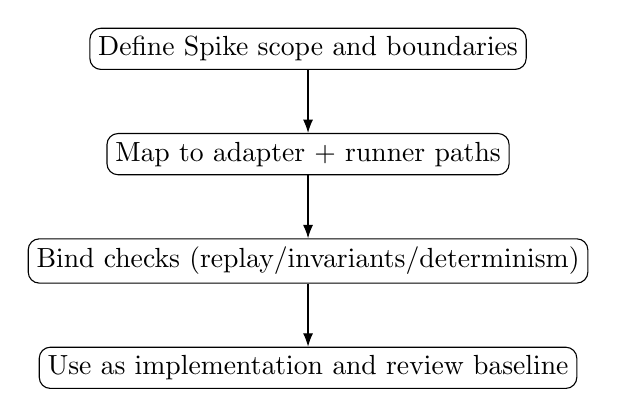
\begin{tikzpicture}[node distance=8mm and 12mm]
\node[box] (a) {Define Spike scope and boundaries};
\node[box, below=of a] (b) {Map to adapter + runner paths};
\node[box, below=of b] (c) {Bind checks (replay/invariants/determinism)};
\node[box, below=of c] (d) {Use as implementation and review baseline};
\draw[line] (a) -- (b);
\draw[line] (b) -- (c);
\draw[line] (c) -- (d);
\end{tikzpicture}
\caption{Spike README Scope Flow}
\end{figure}

\end{document}
